\chapter{O Algoritmo de Cripto-Compressão GMPR}
\label{cap3}

O algoritmo de cripto-compressão \gmpr foi desenvolvido pela \textit{Sheffield Hallam University} em MATLAB~\cite{shu13715}. Neste projeto de trabalho de conclusão de curso, este algoritmo será reescrito em C++ para que seja possível paralelizá-lo.

O algoritmo \gmpr foi desenvolvido com o foco em imagens, sendo superior em qualidade em relação ao conhecido formato \jpeg e com qualidade equivalente ao formato \jpegg. A Tabela~\ref{tab:gmprjpeg} mostra uma comparação do algoritmo \gmpr com os formatos \jpeg e \bmp para imagens 3D.

Ele utiliza a \dct e um algoritmo de minimização de matrizes no estágio de compressão, além de um novo método concorrente de busca binária no estágio de descompressão. Os principais passos do algoritmo de compressão consistem em dividir a imagem em blocos e aplicar a \dct para cada bloco, aplicar o algoritmo de minimização de matrizes nos coeficientes \texttt{AC} de cada bloco, reduzindo a matriz para 1/3 do tamanho, construir uma \lut para permitir a recuperação dos dados originais no estágio de descompressão, aplicar um delta na lista de coeficientes \texttt{DC} e aplicar a codificação aritmética nos resultados. O estágio de descompressão utiliza a \lut e o algoritmo de busca binária para recuperar todos os coeficientes \texttt{AC}, enquanto os coeficientes \texttt{DC} são recuperados revertendo a codificação aritmética, e, finalmente, a \dct inversa recupera a imagem original \cite{shu13715}. A Figura~\ref{fig:gmprcompression} ilustra o processo de compressão.

\begin{table}[t]
\centering
    \begin{tabular}{| l | l | l | l |}
    \hline
        Imagem & \bmp & \jpeg & \gmpr \\ \hline
        Maçã & 336 MB & 52.4 MB & 0.929 MB \\ \hline
        Estátua & 366 MB & 58.5 MB & 0.916 MB \\ \hline
        Rosto & 200.7 MB & 45.5 MB & 0.784 MB \\ \hline
    \end{tabular}
    \caption{Compressão de Imagens 3D.}\label{tab:gmprjpeg}
\end{table}


\section{Compressão}

Primeiramente a imagem é dividida em blocos de tamanho \texttt{n}, e então é aplicada a \dct em cada bloco. Cada bloco consiste de coeficientes \texttt{DC}, que são o valor médio do bloco, e os demais coeficientes, chamados \texttt{AC}. A \dct, um processo sem perdas e reversível, serve para identificar redundâncias na imagem, ou seja, pixeis muito semelhantes em relação aos seus vizinhos.

Em seguida é aplicado o algoritmo de minimização de matrizes na lista de coeficientes \texttt{AC}, eliminando todos os zeros, que geralmente são muitos, reduzindo seu tamanho e produzindo o vetor minimizado. São definidas 3 chaves que irão multiplicar cada 3 entradas deste vetor minimizado, e então os 3 valores são somados, ou seja, cada 3 valores do vetor é transformado em apenas 1, reduzindo o tamanho para 1/3 do original, produzindo o vetor minimizado codificado.

A etapa de descompressão inicia na recuperação dos coeficientes \texttt{DC}, revertendo a codificação aritmética. Os coeficientes \texttt{AC} são recuperados através da busca binária, utilizando as 3 chaves geradas na compressão é possível recuperar o vetor minimizado, decodificando-o.

Em seguida os coeficientes \texttt{DC} a \texttt{AC} são combinados, recolocando todos os zeros que foram removidos na compressão, e em seguida aplicando a \dct inversa para recuperar a imagem original \cite{shu13715}.

\section{Criptografia}

De modo geral, o algoritmo \gmpr inicia a etapa de cifragem obtendo o texto plano e convertendo-o para \texttt{ASCII}. Em seguida é obtida uma lista dos caracteres contidos no arquivo, sem repetir nenhum. Por exemplo: o texto ``abac'' irá gerar uma lista contendo os caracteres ``abc'', não incluindo o caractere ``a'' duas vezes.

\begin{figure}[t]
    \centering
    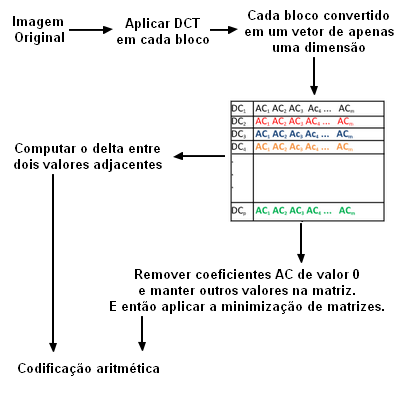
\includegraphics{Images/GMPRCompression.png}
    \caption{Estágio de Compressão do GMPR}
    \label{fig:gmprcompression}
\end{figure}

São geradas 3 chaves aleatórias. A partir disso é gerada uma lista chamada \texttt{nCoded}, na qual a cada 3 caracteres do texto é gerado 1 elemento codificado usando as chaves geradas. O texto ``abac'' geraria 2 elementos nessa lista, pois ``aba'' seria codificado no primeiro elemento e ``c'' codificado no segundo elemento;

É criado um vetor chamado \texttt{codedvector} que é formado pelas 3 chaves, pela lista única de caracteres e pela lista \texttt{nCoded}. Em seguida o texto final codificado é gerado.

\begin{figure}[t]
    \centering
    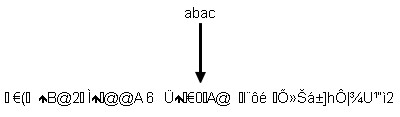
\includegraphics{Images/CifraGMPR.jpg}
    \caption{Binário gerado pelo algoritmo GMPR}\label{fig:gmpr}
\end{figure}

Para decifrar o conteúdo e obter o arquivo original, o algoritmo começa obtendo o texto cifrado e transformando-o em um vetor. Em seguida são extraídas as 3 chaves usadas no processo de cifragem, a lista única de caracteres e a lista \texttt{nCoded}. Por fim, o conteúdo é decodificado.

Se o arquivo cifrado com o algoritmo \gmpr for aberto em algum editor de texto será mostrado algo parecido com o exemplo da Figura~\ref{fig:gmpr}. As seções a seguir apresentam os pseudo-códigos das etapas de cifragem e decifragem do algoritmo.

\subsection{Algoritmo de Cifragem}
		
\begin{algorithm}[t]
\begin{algorithmic}[1]
\footnotesize
    \vspace{0.2em}
    \State $nData \gets$ \Call{abrirArquivoOriginal}{}
    \vspace{0.5em}
    \For{$i$ \textbf{from} $0$ \textbf{to} $nData.tamanho()$}
    \vspace{0.2em}
        \If{$!(nLimited \supset nData[i])$}
            \vspace{0.2em}
            \State \Call{adicionarElemento}{$nLimited$, $nData[i]$}
        \EndIf
    \EndFor
    \vspace{0.5em}
    \State $K[0] \gets$ \Call{rand}{} \% 1001
    \State $K[1] \gets$ (\Call{rand}{} \% 11) * 2 * $maxvalue$
    \State $K[2] \gets$ $K[1]$ * $maxvalue$ * (\Call{rand}{} \% 11)
    \vspace{0.5em}
    \While{$i$ <= $nData.tamanho()$}
        \vspace{0.2em}
        \State $nCoded[i] \gets K[0]*nData[i] + K[1]*nData[i+1] + K[2]*nData[i+2]$
        \State $i \gets i + 3$
    \EndWhile
    \vspace{0.5em}
    \State \Call{adicionarElemento}{$codedvector$, $K$}
    \State \Call{adicionarElemento}{$codedvector$, $nLimited.tamanho()$}
    \State \Call{adicionarElemento}{$codedvector$, $nCoded.tamanho()$}
    \State \Call{adicionarElemento}{$codedvector$, $nLimited$}
    \State \Call{adicionarElemento}{$codedvector$, $nCoded$}
    \vspace{0.5em}
    \State string $msg \gets$ \Call{paraString}{$codedvector$}
    \vspace{0.5em}
    \State $stats \gets$ \Call{obterListaIntervaloProbabilidades}{}
    \For{$i$ \textbf{from} $0$ \textbf{to} $nData.tamanho()$}
        \vspace{0.2em}
        \State \Call{AplicaProbabilidades}{$nData[i]$, $stats$}
    \EndFor
    \vspace{0.5em}
    \State \Call{EscreverDisco}{$stats$}
\end{algorithmic}
\caption{Cifragem}
\label{algorithm: gmprc}
\end{algorithm}

Nas linhas 2 a 4 é criada e preenchida a \texttt{nLimited}, uma lista contendo todos os caracteres únicos do texto plano. 

Em seguida as 3 chaves aleatórias são geradas nas linhas 5 a 7. \texttt{K[0]} é gerada entre 0 e 1000. \texttt{K[1]} gera um valor entre 0 e 10 e depois multiplica pelo dobro do maior caractere do texto plano. \texttt{K[2]} gera um valor entre 0 e 10, multiplica pela chave \texttt{K[1]} e depois multiplica pelo maior caractere do texto plano.

Nas linhas 8 a 10 é criada e preenchida a \texttt{nCoded}, uma lista que contém as chaves \texttt{K} multiplicadas pelo texto plano. Nas linhas 11 a 15 é criado e preenchido o \texttt{codedvector}, um vetor que contém as chaves \texttt{K}, o tamanho da lista \texttt{nLimited}, o tamanho da lista \texttt{nCoded}, o conteúdo da lista \texttt{nLimited} e o conteúdo da lista \texttt{nCoded}.

Na linha 16 é convertido o vetor \texttt{codedvector} para \texttt{string}.

Na linha 17 é obtida uma lista de intervalos de probabilidades para cada símbolo do texto plano. Em seguida são aplicados os intervalos à cada elemento do texto e adicionados ao texto final codificado nas linhas 18 e 19. Por fim o arquivo é salvo em disco na linha 20.

\subsection{Algoritmo de Decifragem}

\begin{algorithm}[t]
\begin{algorithmic}[1]
\footnotesize
    \vspace{0.2em}
    \State $msg \gets$ \Call{ArDecodeFile}{}
    \vspace{0.5em}
    \State $data \gets$ \Call{paraVetor}{$msg$}
    \vspace{0.5em}
    \State $K[0] \gets data[0]$
    \State $K[1] \gets data[1]$
    \State $K[2] \gets data[2]$
    \vspace{0.5em}
    \State $nL \gets data[3]$
    \vspace{0.5em}
    \State $nC \gets data[4]$
    \vspace{0.5em}
    \For{$i$ \textbf{from} $5$ \textbf{to} $5+nL$}
        \vspace{0.2em}
        \State $nLimited[i] \gets data[i]$
    \EndFor
    \vspace{0.5em}
    \For{$i$ \textbf{from} $5+nL+1$ \textbf{to} $5+nL+1+nC$}
        \vspace{0.2em}
        \State $nCoded[i] \gets data[i]$
    \EndFor
    \vspace{0.5em}
    \State $ultimaPos \gets data.tamanho()$
    \For{$r$ \textbf{from} $0$ \textbf{to} $ultimaPos$}
        \vspace{0.2em}
        \For{$i$ \textbf{from} $0$ \textbf{to} $nL$}
            \vspace{0.2em}
            \For{$j$ \textbf{from} $0$ \textbf{to} $nL$}
                \vspace{0.2em}
                \For{$k$ \textbf{from} $0$ \textbf{to} $nL$}
                    \vspace{0.2em}
                    \If{$data[r] == K[0]*nLimited[i] + K[1]*nLimited[j] + K[2]*nLimited[k]$}
                        \vspace{0.2em}
                        \State $nDecoded[3*r+0] \gets nLimited[i]$
                        \State $nDecoded[3*r+1] \gets nLimited[j]$
                        \State $nDecoded[3*r+2] \gets nLimited[k]$
                    \EndIf
                \EndFor
            \EndFor
        \EndFor
    \EndFor
    \vspace{0.5em}
    \State \Call{EscreverDisco}{$nDecoded$}
\end{algorithmic}
\caption{Decifragem}
\label{algorithm: gmprd}
\end{algorithm}

Na linha 1 a rotina \texttt{ArDecodeFile} abre o arquivo cifrado, faz uma leitura do cabeçalho e gera a lista de probabilidades que será usada para decodificar o arquivo. Em seguida a \texttt{string} é convertida para vetor na linha 2.

Nas linhas 3 a 5 são obtidas as 3 chaves que foram usadas para cifrar. O tamanho da lista de caracteres únicos \texttt{nLimited} é obtido na linha 6 e seu conteúdo obtido nas linhas 8 e 9. O tamanho da lista \texttt{nCoded}, que contém as chaves \texttt{K} multiplicadas pelo texto plano, é obtido na linha 7 e seu conteúdo obtido nas linhas 10 e 11.

Nas linhas 12 a 20 o texto é decodificado, obtendo o conteúdo original. É feito o processo inverso da geração da lista \texttt{nCoded} no processo de cifragem, e quando o elemento codificado é encontrado então ele é salvo na lista \texttt{nDecoded}. Por fim o arquivo é salvo em disco.